\section{Image processing and information extraction}\label{sec:improc}

\subsection{Simple calculus with channels}\label{ssec:calculus}

The Band Math application, \textbf{otbBandMath-cli}, provides a simple and efficient way to perform band operations. The command line application and the corresponding Monteverdi module (shown in the section \ref{Band_math module}) are based on the same standards. It computes a band wise operation according to a user defined mathematical expression. The following code computes the absolute difference between first bands of two images:

\begin{verbatim}
otbBandMath-cli -ims input_image_1 input_image_2 
                -exp "abs(im1b1 - im2b1)"
                -out output_image
\end{verbatim}

The naming convention "im[x]b[y]" designates the yth band of the xth input image.

The Band Math application embeds built-in operators and functions (listed \href{http://muparser.sourceforge.net/mup_features.html#idDef2}{here}), allowing a vast choice of possible operations. 

\subsection{Classification}\label{ssec:classification}

The aim of the new SVM classification framework is to provide a supervised pixel-wise classification chain based on learning from multiple images. It supports huge images through streaming and multi-threading.
The classification chain will perform a SVM training step based on the intensities of each pixel as features. Please note that the images will have the same number of bands to be comparable.

\subsubsection{Statistics estimation}
In order to make these features comparable between each images, the first step is to estimate the input images statistics. These statistics will be used to center and reduce the intensities (mean of 0, standard deviation of 1) of samples based on the vector data produced by the user. To do so, the \textbf{otbEstimateImagesStatistics} tool can be used :

\begin{verbatim}
otbEstimateImagesStatistics-cli -in  list_of_input_images 
                                -out statistics.xml
\end{verbatim}

This tool will compute each band mean, compute the standard deviation based on pooled variance of each band and finally export them to an XML file.

The features statistics XML file will be an input of the following tools. 

\subsubsection{Building a training data set}

The chain is supervised : one has to build a training set with positive examples of different objects of interest. This can be done with Monteverdi Vectorization module (Fig.\ref{fig:vectoModuleDataSetCreation}), by building a VectorData containing polygons centered on occurrences of the different objects of interest. This operation will be reproduced on each image used as input of the training function.

Please note that the positive examples in the vector data should have a Class field with a label higher than 1 and coherent in each different images. 

\begin{figure}
  \center
  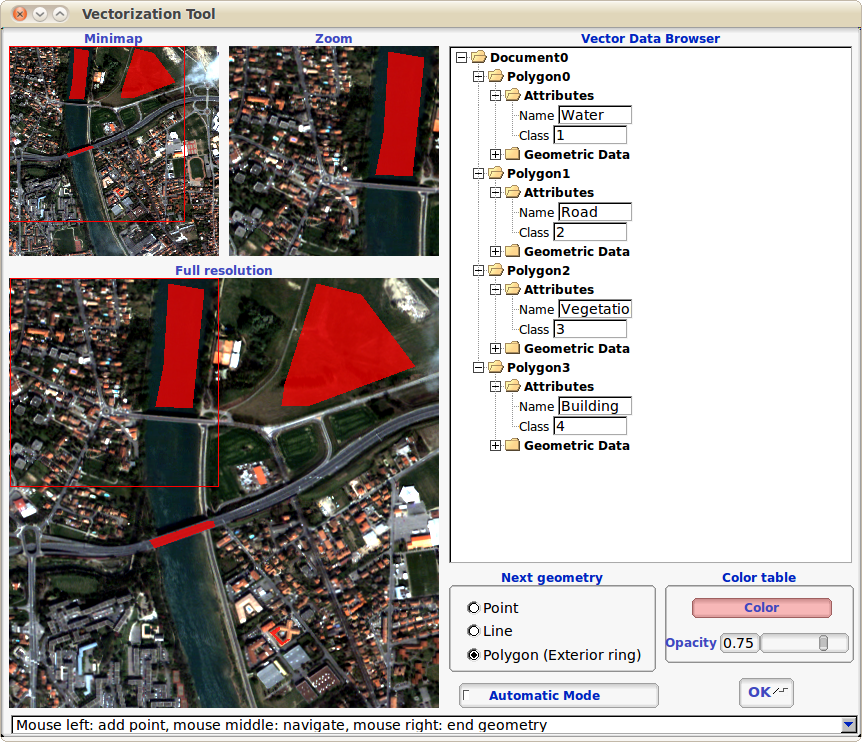
\includegraphics[width=1\textwidth]{../Art/MonteverdiImages/monteverdi_vectorization_module_for_classification.png}
  \itkcaption[GUI of the vectorization module with data for classification chain]{A training data set builded with the vectorization monteverdi module.}
  \label{fig:vectoModuleDataSetCreation}
\end{figure}

You can generate the vector data set with QGIS software for example. The \app should be able to transform the vectordata into the image coordinate system. 

\subsubsection{Training data set}

Once images statistics have been estimated, the learning scheme is the following:
\begin{enumerate}
  \item For each input image:
  \begin{enumerate}
    \item Read the region of interest (ROI) inside the shapefile,
    \item Generate validation and training data within the ROI,
    \item Add the vectors respectively to the training samples set and the validation samples set.
  \end{enumerate}
  \item Increase the size of the training samples set and balance it by generating new noisy samples from the previous ones,
  \item SVM learning with this training set
  \item Performances estimation of the SVM classifier on the validation samples set (confusion matrix, precision, recall).
\end{enumerate}

These steps can be performed by the \textbf{otbTrainImagesClassifier} command-line using the following:

\begin{verbatim}
otbTrainImagesClassifier-cli -is  images_statistics.xml 
                             -in  list_of_input_images 
                             -vd  list_of_positive_examples_shapefiles
                             -out model.svm
                             -b
\end{verbatim}

Some options are available:
\begin{itemize}
\item -dem \textit{a DEM directory to keep accurate the vectordata reprojection}
\item -m   \textit{margin value}
\item -k   \textit{svm kernel (0 = LINEAR (default), 1 = RBF,  2 = POLY, 3 = SIGMOID) }
\item -opt \textit{use svm parameters optimization}
\item -mt  \textit{maximum training samples size} 
\item -mv  \textit{maximum validation samples size}
\item -vrt \textit{ratio validation training}
\end{itemize}

\subsubsection{Validate the classification model}
It is also possible to estimate the SVM model performance with a new validation sample set and another image with the following application.
It will compute the global confusion matrix and precision, recall and F-score of each class based on the \href{http://www.orfeo-toolbox.org/doxygen-current/classotb_1_1ConfusionMatrixCalculator.html}{ConfusionMatrixCalculator} class.
It is done by \textbf{otbValidateImagesClassifier}:

\begin{verbatim}
otbValidateImagesClassifier-cli -is  images_statistics.xml
                                -svm model.svm
                                -in  input_image
                                -vd  list_of_positive_examples_shapefiles
\end{verbatim}

You can save these results with the option -out output filename. You can also set a DEM repository (-dem) to keep the vectordata reprojection accurate.

\subsubsection{Using the classification model} 
Once the classifier has been trained, one can apply the model to classify pixel inside defined classes on a new image using the \textbf{otbImageSVMClassifier} tool:

\begin{verbatim}
 otbImageSVMClassifier-cli -is  images_statistics.xml
                           -svm model.svm 
                           -in  input_image
                           -out labeled_image
\end{verbatim}

You can set an input mask to limit the classification to the mask area with value \textgreater 0.

\subsubsection{Fancy classification results}

In order to get an RGB classification map instead of greylevel labels, one can use the \textbf{otbLabeledImageColorMapping} tool. This tool will replace each label with an 8-bits RGB color specificied in a mapping file. The mapping file should look like this :

\begin{verbatim}
# Lines beginning with a # are ignored
1 255 0 0
\end{verbatim}

In the previous example, 1 is the label and 255 0 0 is a RGB color (this one will be rendered as red). To use the mapping tool, enter the following :

\begin{verbatim}
otbLabeledImageColorMapping-cli -in  labeled_image 
                                -out color_image
                                -ct  mapping_file
\end{verbatim}

\subsubsection{Example}
We take 4 classes: water, roads, vegetation and buildings with red roof.
Data are available in the OTB-Data \href{http://hg.orfeo-toolbox.org/OTB-Data/file/0fed8f4f035c/Input/Classification}{repository} and this image is produced with the commands inside this \href{http://hg.orfeo-toolbox.org/OTB-Applications/file/3ce975605013/Testing/Classification/CMakeLists.txt}{file}. 

\begin{figure}[!h]
  \center
  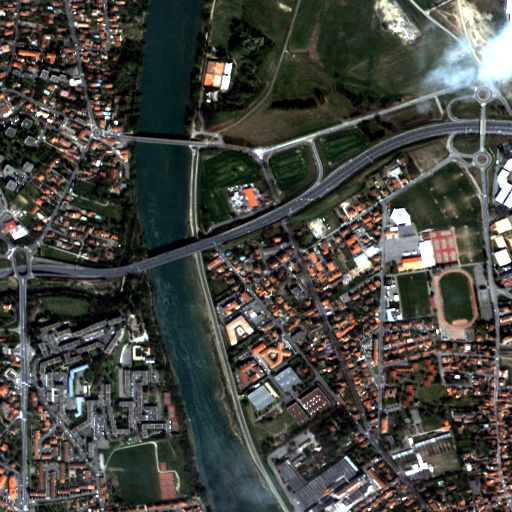
\includegraphics[width=0.3\textwidth]{../Art/MonteverdiImages/classification_chain_inputimage.jpg}
  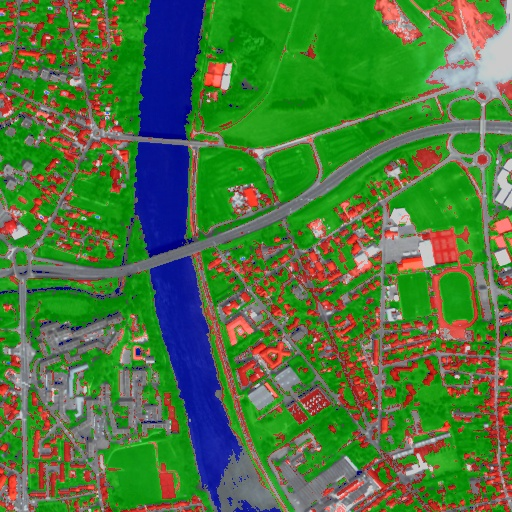
\includegraphics[width=0.3\textwidth]{../Art/MonteverdiImages/classification_chain_fancyclassif_fusion.jpg}
  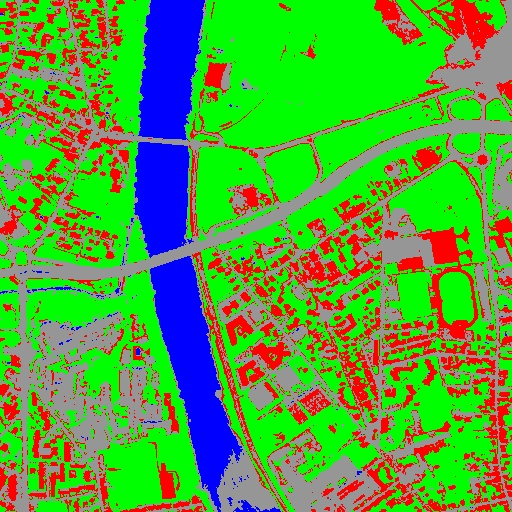
\includegraphics[width=0.3\textwidth]{../Art/MonteverdiImages/classification_chain_fancyclassif.jpg}}
  \itkcaption[ExampleSVMCalssif]{From left to right: Original image, result image with fusion (with monteverdi viewer) of original image and fancy classification and input image with fancy color classification from labeled image.}
  \label{fig:MeanShiftVectorImageFilter}
\end{figure}



%\subsection{Segmentation}\label{ssec:segmentation}
%todo.

%\subsection{Change detection}\label{ssec:changedetection}
%todo.

%\subsection{Object-based image analysis}\label{ssec:obia}
%todo.

\subsection{Dempster Shafer based Classifier Fusion}\label{ssec:classifierfusion}

This framework is dedicated to, starting from the result of a detection (for example a road extraction), enhance the results fiability by using a classifier fusion based validation algorithm. Using a set of descriptor, the processing chain validates or invalidates the input geometrical features.

\subsubsection{Prequel: Road Extraction}

The first step of this recipe is to produce an interesting and adapted input. The otbRoadExtractionApplication,  included in the OTB-Applications package, provides a set of geometrical features that can be used as input of the following process. This is only an example, the Dempster-Shafer framework was not designed specificaly to be used with otbRoadExtractionApplication but it is a good example of what the input should be like.

\subsubsection{Fuzzy Model (requisite)}

Perform the fuzzy model estimation (once by use case: descriptor set / Belief support / Plausibility support).
Inputs:
\begin{itemize}
\item a vector data of positive samples enriched according to the "Compute Descriptors" part
\item a vector data of positive samples enriched according to the "Compute Descriptors" part
\item a support for the Belief computation
\item a support for the Plausibility computation
\item a initialization model (xml file) or a descriptor name list (listing the descriptor to be included in the model)
\end{itemize}
Output:
\begin{itemize}
\item a FuzzyModel.xml file containing the model
\end{itemize}
Usage:

\begin{verbatim}
 otbDSFuzzyModelEstimation-cli -psin     PosSamples.shp 
                               -nsin     NegSamples.shp 
                               -BelSup   "ROADSA" 
                               -PlaSup   "NONDVI" "ROADSA" "NOBUIL" 
                               -DescList "NONDVI" "ROADSA" "NOBUIL" 
                               -out      FuzzyModel.xml
\end{verbatim}

FuzzyModel.xml contains the optimal model to perform the classifier fusion.

\subsubsection{First Step: Compute Descriptors}

The First step in the classifier fusion based validation is to compute, for every studied polyline, the choosen descriptors. In this context, the otbComputePolylineFeatureFromImage application can be used for a large panel of descriptors.
Inputs:
\begin{itemize}
\item an image (of the sudied scene) corresponding to the choosen descriptor (NDVI, building Mask...)
\item a vector data containing polyline of interest
\item a formula ("b1 \textgreater 0.4", "b1 == 0") where b1 is the standard name of input image first band
\item a field name corresponding to the descriptor codename (NONDVI, ROADSA...)
\end{itemize}
Output:
\begin{itemize}
\item a vector data containing polylines with a new field containing the descriptor value
\end{itemize}
Usage: To add the "NONDVI" descriptor to an input VectorData ("inVD.shp") corresponding to the percentage of pixel along a polyline that verifies the formula that have a NDVI \textgreater 0.4 :

\begin{verbatim}
 otbComputePolylineFeatureFromImage-cli -img   NDVI.TIF 
                                        -vdin  inVD.shp 
                                        -expr  "b1 > 0.4" 
                                        -field "NONDVI" 
                                        -out   VD_NONDVI.shp
\end{verbatim}

where NDVI.TIF is the ndvi mono band image of the studied scene.
This step must be repeated for each choosen descriptor

\begin{verbatim}
 otbComputePolylineFeatureFromImage-cli -img   roadSpectralAngle.TIF  
                                        -vdin  VD_NONDVI.shp 
                                        -expr  "b1 > 0.24"
                                        -field "ROADSA" 
                                        -out   VD_NONDVI_ROADSA.shp
\end{verbatim}

\begin{verbatim}
 otbComputePolylineFeatureFromImage-cli -img   Buildings.TIF 
                                        -vdin  VD_NONDVI_ROADSA.shp 
                                        -expr  "b1 == 0" 
                                        -field "NOBUILDING" 
                                        -out   VD_NONDVI_ROADSA_NOBUIL.shp
\end{verbatim}

Both NDVI.TIF and roadSpectralAngle.TIF can be produced using Monteverdi Feature Extraction capabilites, and Buildings.TIF can be generated using Monteverdi Rasterization module.
From now on, VD\_NONDVI\_ROADSA\_NOBUIL.shp contains three descriptor fields. It will be used in the following parts.

\subsubsection{Second Step: Feature Validation}

The final application which, using the Dempster-Shafer theory, will validate or unvalidate the studied samples
Inputs:
\begin{itemize}
\item an enriched vector data VD\_NONDVI\_ROADSA\_NOBUIL.shp
\item a support for the Belief computation
\item a support for the Plausibility computation
\item a fuzzy model FuzzyModel.xml
\end{itemize}
Output:
\begin{itemize}
\item a vector data containing only the validated samples
\end{itemize}
\begin{verbatim}
 otbVectorDataDSValidation-cli -in      extractedRoads_enriched.shp 
                               -descMod FuzzyModel.xml 
                               -out     validatedSamples.shp
\end{verbatim}

